
\def\year{2017}\relax
%File: formatting-instruction.tex
\documentclass[letterpaper]{article}
\usepackage{aaai17}
\usepackage{times}
\usepackage{helvet}
\usepackage{courier}
\usepackage[table]{xcolor}
\usepackage{graphicx}
\usepackage{amssymb,amsmath,amsthm,amsfonts}
\usepackage[vlined,ruled,linesnumbered]{algorithm2e}

\usepackage{algpseudocode}
\usepackage{float}
\usepackage{tikz}
\usepackage{color}
\usepackage{calc}
\usepackage{subfig}

\usepackage{booktabs}
\usepackage{multirow}


\frenchspacing

\setlength{\pdfpagewidth}{8.5in}
\setlength{\pdfpageheight}{11in}

\pdfinfo{
/Title (Towards Backbone Computing: A Greedy-Whitening Based Approach)
/Author ()}
\setcounter{secnumdepth}{1}


\newcommand{\X}{\mathcal{X}}
\newcommand{\g}{\mathcal{G}}
\newcommand{\var}{\textsf{var}}
\newcommand{\Lit}{\textsf{lit}}

\newcommand {\SAT}{\textsf{SAT}}
\newcommand {\MUC}{\textsf{MUC}}
\newcommand{\degr}{\textsf{d}}
\newcommand{\BL}{\textsf{BL}}
\newcommand{\BLap}{{\sf \widehat{BL}}}
\newcommand{\NBLap}{{\sf \overline{BL}_\downharpoonright}}
\newcommand{\BV}{\textsf{BV}}
\newcommand{\HDBS}{\textsf{HDBS}\xspace}

\newcommand{\tool}{{\sc Bone}\xspace}
\newcommand{\NBV}{\overline{\textsf{BV}}}
\newcommand{\NBL}{\overline{\textsf{BL}}}
\newcommand{\NBC}{\overline{\textsf{BC}}}

\newcommand{\HBL}{{\sf HBL}\xspace}

\newcommand{\cls}{\textsf{cls}}
\newcommand{\NB}{{\bf NB$\downharpoonright$}}
\newcommand{\MBNB}{{\bf MBNB$\downharpoonright$}}
\newcommand{\HBNB}{{\bf HBNB$\downharpoonright$}}
\newtheorem{theorem}{Theorem}
\newtheorem{lemma}{Lemma}
\newtheorem{corollary}{Corollary}
\newtheorem{definition}{Definition}
\newtheorem{example}{Example}
\newtheorem{remark}{Remark}

 \begin{document}
% The file aaai.sty is the style file for AAAI Press
% proceedings, working notes, and technical reports.
%
\title{Towards Backbone Computing: A Greedy-Whitening Based Approach}

%\author{Yueling Zhang \\ {\bf Min Zhang} \\ {\bf Geguang Pu} \\ Shanghai Key Laboratory of Trustworthy Computing \\ National Research Center of Trustworthy Embedded Software \\ East China Normal University, China  \\ {ylzhang, mzhang, ggpu} @sei.ecnu.edu.cn
%Fu Song \\ School of Information Science and Technology, ShanghaiTech University \\ songfu@shanghaitech.edu.cn}

% \author{Yueling Zhang \\ {\bf Min Zhang} \and {\bf Geguang Pu}
% \\ Shanghai Key Laboratory of Trustworthy Computing
% \\ National Research Center of Trustworthy Embedded Software
% \\ East China Normal University, China
% \\ \{ylzhang, mzhang, ggpu\}@sei.ecnu.edu.cn
% \And Fu Song
% \\ School of Information Science and Technology
% \\ ShanghaiTech University, China
% \\ songfu@shanghaitech.edu.cn
% \AND Jianwen Li
% \\ jwli@sei.ecnu.edu.cn
%}

\maketitle

\begin{abstract}
Backbone is widely used in random SAT solving, \#SAT and planning, etc.
In this paper, we propose a greedy-whitening based approach for computing backbone of propositional Boolean formulae.
We present a greedy-based algorithm with two heuristic searching strategies to compute an under-approximation of non-backbone and
a whitening-based algorithm to compute an approximation of backbone.
The exact backbone is computed by applying iterative test backbone on the approximations.
We implemented our approach in a tool \tool and conducted experiments on instances from Industrial and Random tracks of SAT Competitions
between 2002 and 2015. Experimental results demonstrate that \tool is more efficient than
to the state-of-the-art tool cb100. Moreover, \tool reduces 40\% running time for hard random formulae and cut off 11\% running time for industrial formulae comparing to cb100.

%For the formulae that with disperse backbones, our approach is able to compute an estimation of literals that are highly likely to be %backbones and applied backbones extraction algorithms in the following steps.
%Experiments show the efficiency of the approach using satisfiable instances from SAT Competition, including both SAT track and Maximal %Satisfiability Sub-formulae(MSS) extracted from UNSAT track. Moreover, compared with state-of-the-art approach proposed in 2015, our %approaches has advantages in hard formulae and MSS formulae.
\end{abstract}


\section{Introduction}

Backbones are firstly generalized from the coloring problem. A pair of nodes are backbones if they always have the same color in every possible k-coloring\cite{WTS2001}.

In satisfiability problem, given a formulae $\Phi$, an truth assignment is a map from boolean variables to literals appeared in $\Phi$. In an assignment, a literal can only be assigned as TRUE or FALSE. Given an assignment $\lambda$, if there exist at least one literal in a clause $\phi\in\Phi$ that has been assigned as TRUE according to $\lambda$, $\phi$ is called to be satisfied by $\lambda$. If there exists a $\lambda$ that satisfy every clause $\phi\in\Phi$, $\lambda$ is a model or a satisfied assignment of $\Phi$.
Backbones of a propositional formula $\Phi$ is a cluster of literals that are TRUE in every model of $\Phi$\cite{BCJ2001,KPJ2005}.

Backbones have been studied in random 3-SAT problems \cite{DOG2001}, optimization problems\cite{CJG2001,KPS2005,WTS2001}, as well as Maximal Satisfiability(MSS) problems\cite{MM2005}.
As shown in \cite{ZWR2003}, backbones are applied to local minima of Walksat and improves the performance of Walksat by making biased moves in a local search. Another similar application of backbones information is shown in \cite{ZWL2005}, in this experiment, backbones information significantly contributes to the acceleration of Lin-Kernighan(LK) local search family algorithms when dealing with Travel Salesman Problem(TSP).
A more recent application of backbones arises in \cite{Z11}. A number of backbones extracting approaches are proposed and applied to post silicon fault localisation. The results show that backbones extracting using SAT solvers are suitable for large scale applications with only a little SAT solver calls.

As shown above, finding backbones is the key in many practical applications, such as planning problem and constraint satisfaction problem. It has been proved that backbones computing is a co-NP problem\cite{Jan10}, which have rise huge challenges.
A number of backbones extraction algorithms have been proposed in recent years. All state-of-the-art backbones extraction approaches employ SAT solvers, MiniSAT\cite{MINISAT} for most of them.
Implicant enumeration\cite{MK2002,RSF2004} enumerates implicants of formula $\Phi$ one by one and updates the backbones estimation in each iteration. The negation of an implicant is added to $\Phi$ in order to avoid finding the same implicant. For an implicant $\lambda$, the negation of $\lambda$ is $\bigvee_{l\in\lambda}\neg l$. Standard implicants reducing techniques can be applied to mitigate the size of blocking clauses. It have to enumerate all models of $\Phi$ before the algorithm terminates, which is unnecessary costly.

Zhu et al, proposed an iterative SAT testing algorithm \cite{Z11}. The algorithm maintains an estimation of backbones $\Phi_\BL$. The negation of $\Phi_\BL$ is the disjunction of each complementing literals in backbones estimation, i.e., $\neg\Phi_\BL=\bigvee_{\neg l}, l\in\Phi_\BL$. In each iteration, a clause that formed by $\neg \Phi_\BL$ conjuncted to $\Phi$ and formed $\Phi'$. If $\Phi'$ is satisfiable, it means that at least one non-backbone is in the backbone estimation, estimation is refined by removing the non-backbone literal. The process is repeated until $\Phi'$ is not satisfiable any longer. Along with the estimation, the clauses number of $\Phi'$  is monotone increasing due to the continuously disjunction in each iteration, which dramatically promote the complexity of $\Phi'$. In other words, for each iteration, it takes longer CPU time than the last iteration.

The Core Based Algorithm presented in \cite{JLM15} is stable and effectiveness. It considers complementing of the model as assumptions input for SAT solver in each iteration. If $\Phi$ is unsatisfied under given assumptions, a core is returned by SAT solver to indicate reasons. According to the implementation of MiniSAT 2.2 \cite{MINISAT}, the reason is a part of the given assumptions. Whenever there is exactly one literal in the reason, the literal is a backbone. If there is more than one literal in the reason, they will be marked as visited. If every literal in an iteration is visited, iterative SAT testing will be invoked to test the rest of unmarked literals. According to the author, for the lower percentages of backbones, Core Based Algorithms are significantly better. When the percentage of backbone is over 25\%, Core Based Algorithm behave very similarly Iterative SAT Testing Algorithm.

Revisited previous researches, backbones computing of low density backbones formulae is quiet efficiencies and efficiency. In this paper, we focus on the hard instance, proposed a novel approach to spot non-backbones ahead and to estimate backbones. Instead of accumulating clauses to formula like Iterative SAT testing does, we test the literals one by one by leveraging assumptions. Assumptions are a group of literals. We consider assumptions as a kind of constraint input, it means that the literals in assumptions must be assigned to true in an assignment. If there exists a model $\lambda$ such that it satisfy every literals in assumptions, the formula is satisfied under these assumptions. According to the satisfiability theory, assumptions are equivalence to clauses that only contains the assumption literal. Compared with clauses conjunction, assumptions won't increase the complexity of formula since no clauses are added to the formula. Also, assumptions is more suitable for iterative SAT testing since it can be reset in each iteration.

Using variables clauses coverage analysis, a group of non-backbone literals and an estimation of backbones are obtained, refereed as $\NBL_u$ and $\HDBS$, respectively. For each literals in $\HDBS$, Minisat with assumptions will be evoked. The only assumption in each iteration is the current testing literal. If Minisat returns false, the literal is a backbone, it will be conjuncted with the original formula to simplify it.

The approach leveraging Whitening Algorithm and other pervious backbones computing algorithms, designed and implemented a Multi Estimation Based Algorithms (MEB) , experiments are conducted to evaluate MEB, results showed that MEB is compatible with Core Based Algorithm when dealing with low density backbones formulae. For hard formulae with dense backbones, MEB outperforms Core Based Approach considering the total SAT solver time and SAT calls number.
Compared with Core Based Algorithm which directly calculate backbones. MEB estimate non-backbone literals and backbone literals ahead.
Unlike the Iterative SAT Testing approach, the estimation doesn't need to rely on SAT solvers. Only one SAT solver call is needed during the estimation process. 
%FCB will first compute the under-approximation of non-backbone literals, referred as $\NBL_u$ in $O(n^2)$ time. With the $\NBL_u$ information, a group of literals with dense backbones will be estimated in polynomial time, refereed as $\HDBS$.
%Iterative SAT testing per literals of $\HDBS$ will be applied to determine whether a literal is a backbone or not. A backbone literal will be conjuncted with formula as a new unit clause. With several backbones, formula will be simplified\cite{MPA2015}.
Experiments indicate that, the average dense of backbones in $\HDBS$ is over 50\%, which helps MEB to recognize more backbones in less SAT solver calls than CB needs. Especially for hard formulae, MEB will save a large amount of CPU time since it invoking less Minisat than CB does.

This paper is organized as follows.
Section 2 introduces the concept of backbones.
Section 3 relates backbones estimate reducing procedures to Core Based Backbones Extraction Algorithms and evolved to Filter Core Based(FCB) Backbone Extraction Algorithms.
Section 4 presents the experimental evaluation of FCB.
Section 5 makes a conclusion and discusses about future work.

\section{Preliminaries}\label{sec:prel}

We fix a finite set  $\X$ of \emph{Boolean variables}.
A \emph{literal} $l$ is either a Boolean variable $x\in \X$ or its negation $\neg x$.
The negation of a literal $\neg x$ is $x$, i.e., $\neg\neg x=x$.
A \emph{clause} $\phi$ is a disjunction of literals $\bigvee_{i=1}^n l_i$, which may be regarded as
the set of literals $\{l_i\mid 1\leq i\leq n\}$. W.l.o.g., we assume that for every
clause $\phi$, if $l\in\phi$, then $\neg l\not\in \phi$.

A \emph{formula} $\Phi$ over $\X$ is a Boolean combination of variables $\X$.
We assume that formulae are given in conjunctive normal
form (CNF), namely each formula $\Phi$ is a conjunction of clauses $\bigwedge_{i=1}^n\phi_i$ which may be regarded as a set of clauses $\{\phi_i\mid 1\leq i\leq n\}$. Given a formula $\Phi$, let $\var(\Phi)$ (resp. $\Lit(\Phi)$  and $\cls(\Phi)$) denote the set of variables (resp. literals and clauses) used in $\Phi$.
We use $\|\Phi\|$ to denote $\sum_{\phi\in\Phi}|\phi|$.
We use $\neg\Lit(\Phi)$ to denote the set $\{\neg l \mid l\in \Lit(\Phi)\}$.
The \emph{size} $|\Phi|$ of $\Phi$ is the number of literals of $\Phi$.
Given a formula $\Phi$ and a literal $l\in\Lit(\Phi)$,
let $\Phi_{l}\subseteq \Phi$ be the set of clauses $\{\phi\in\Phi\mid l\in\phi\}$.
%and $\Phi_\downarrow$ be the set $\{(l,\Phi_{\downarrow l})\mid l\in \Lit(\Phi)\}$.
%Given a clause $\phi$ of $\Phi$, let $\sharp(\phi,\Phi)$ be the count of occurrence of $\phi$ in the second components of tuples in $\Phi_\downarrow$.
%Given a set of clauses $\Phi_{l_x}$, let $\Phi_{l_x}^0 = \Phi_{\downarrow l}$, let $\Phi_{\downarrow l}^k$, $\Phi_{\downarrow l}^{k-1}\subseteq\Phi_{\downarrow l}^k\subseteq\Phi_{\downarrow 1}^{k+1}\subseteq\Phi (k \geq 1)$ be the set of clauses $\{\phi\in\Phi \mid \exists l\in\Lit(\Phi_{\downarrow l}^{k-1}), \neg l\in\Lit(\phi)\} (k \geq 1)$.

%A \emph{partial assignment} is a partial function $\lambda:\X\rightarrow \{0,1\}$ which assigns to each defined variable a Boolean value. Let $\lambda_x$ denote the partial assignment such that for every $y\in \X$, $\lambda_x(y)=\lambda(x)$ if $x=y$, otherwise $\lambda_x(y)$ is undefined.
%A \emph{complete assignment} is a partial assignment in which all the variables are defined.

An \emph{assignment} is a function $\lambda: \X \rightarrow \{0,1\}$, where $1$ (resp. $0$) denotes true (resp. false).
Given an assignment $\lambda$ and a literal $l$ that is $x$ or $\neg x$, let $\lambda[\neg l]$ be the assignment which is equal to $\lambda$
except for $\lambda[\neg l](x)=\neg \lambda(x)$. Given a set of variables $x=\{x_1,...,x_n\}$, let $\lambda[\neg L]$ denote the assignment
$\lambda[\neg x_1]...[\neg x_n]$.
An assignment $\lambda$ \emph{satisfies} a formula $\Phi$, denoted by $\lambda\models \Phi$, iff assigning $\lambda(x)$ to $x$ for $x\in\var(\Phi)$ makes $\Phi$ true.

An assignment $\lambda$ is a \emph{model} of $\Phi$ if $\lambda\models \Phi$.
Given two models $\lambda_1$ and $\lambda_2$ of $\Phi$, $\lambda_2$ can be \emph{generated} from $\lambda_1$, denoted by $\lambda_1\Rightarrow_\Phi\lambda_2$, if there exists a literal $l$ such that $\lambda_2=\lambda_1[\neg l]$.
Let $\Rightarrow^*_\Phi$ denote the \emph{reflexive transitive} closure of $\Rightarrow_\Phi$.
Formally, for every model $\lambda$ of $\Phi$, $\lambda\Rightarrow^*_\Phi\lambda$ and $\lambda_1\Rightarrow^*_\Phi\lambda_3$ if $\lambda_1\Rightarrow^*_\Phi\lambda_2$ and $\lambda_2\Rightarrow^*_\Phi\lambda_3$.
A \emph{model cluster} $\cl_\Phi(\lambda)$ of $\lambda$ is the set of models $\{\lambda'\mid \lambda\Rightarrow^*_\Phi\lambda'\}$.
A literal $l$ is a \emph{frozen literal} in a model $\lambda$ of $\Phi$,
if $l$ takes the same value in all the models of $\cl_\Phi(\lambda)$. Let $\FL(\Phi,\lambda)$ denote the set of all the frozen literals
in the model $\lambda$ of $\Phi$. %, and $\FL(\Phi)$ denote the intersection of $\FL(\Phi,\lambda)$ for all the models $\lambda$ of $\Phi$.


A formula $\Phi$ is \emph{satisfiable} iff there exists an assignment $\lambda$ such that $\lambda\models \Phi$.
%A variable $x\in\phi$ \emph{satisfies} a formula $\Phi$, denoted by $x\models\Phi$, iff assigning $1$ to $x$ makes with its value $\lambda(x)$.
Given a formula $\Phi$, the \emph{satisfiability problem} is to decide whether $\Phi$ is satisfiable or not.
%Whenever convenient, a formula $\Phi$ is seen as a set $\cls(\Phi)$ of clauses, a clause $\phi$ is seen as a set $\Lit(\phi)$ of literals, and an assignment %$\phi$ is seen as a set of clauses.
%In the rest of this section, we will introduce several technical concepts, amendable to our approach.

\smallskip
%Given an unsatisfiable Boolean formula $\Phi$, an \emph{unsatisfiable core} is a subset of clauses $C\subseteq \cls(\Phi)$ such that
%$\Phi_C$ is still unsatisfiable. An unsatisfiable core $C$ of $\Phi$ is called a \emph{minimal unsatisfiable core} if
%for every $C'\subset C$, $\Phi_{C'}$ is satisfiable. Intuitively, unsatisfiable core is a minimal unsatisfiable core it is unsatisfiable, but removing any of %its clauses makes it satisfiable.

\begin{definition}[Backbone]
\label{def:backbone}
Given a satisfiable formula $\Phi$, a literal $l$ is a \emph{backbone literal} of $\Phi$ iff for all assignments $\lambda$ such that $\lambda\models\Phi$,
$\lambda\models l$. The \emph{backbone} $\BL(\Phi)$ of $\Phi$ is the set of backbone literals of $\Phi$.
\end{definition}


Since a backbone literal takes same value in all the models and a frozen literal takes same value in a model cluster instead of all the models,
we get that:

\begin{proposition}\label{prop:Frozen-backbone}
For any formula $\Phi$ and model $\lambda$ of $\Phi$, $\BL(\Phi)\subseteq\FL(\Phi,\lambda)$.
\end{proposition}


%\begin{definition}[Nonbackbone]
%\label{def:backbone}
%Given a satisfiable formula $\Phi$, a variable $x\in\var(\Phi)$ is a \emph{nonbackbone variable} of $\Phi$ iff there exist two satisfying assignments
%$\lambda_1$ and $\lambda_2$ such that $\lambda_1(x)\neq \lambda_2(x)$.
%A clause $\phi\in \Phi$ is \emph{nonbackbone clause} iff $|\var(\phi)|\geq 2$ and there is a nonbackbone variable of $\Phi$ in $\phi$.
%For an unsatisfiable formula $\Phi$, the set of nonbackbone variables is $\var(\Phi)$.
%\end{definition}
It is known that the backbone $\BL(\Phi)$ for each formula $\Phi$ is unique \cite{JLM15}.
The backbone of an unsatisfiable formula can be defined as an empty set. Therefore, in this work, we focus on satisfiable formulae.
We will use $\NBL(\Phi)$ to denote the set
$\Lit(\Phi)\setminus \BL(\Phi)$.

\begin{theorem}
\label{thm:co-NP}\cite{Jan10}
Given a satisfiable formula $\Phi$ and a literal $l$, deciding whether $l$ is a backbone literal is co-NP-complete.
\end{theorem}

% \begin{definition}[Model]
% Given a satisfied formula $\Phi$, a model $\lambda$ is a truth assignment such that $\lambda\models\Phi$.
% \end{definition}

\begin{definition}[Satisfied literal]
Given a model $\lambda$ of the formula $\Phi$ and a clause $\phi\in\Phi$, for each literal $l\in\phi$, $l$ is a \emph{satisfied literal}
of $\phi$ iff $\lambda\models l$. $l$ is a \emph{unique satisfied literal} of $\phi$ if there is no satisfied literal $l'$ of $\phi\setminus\{l\}$.
\end{definition}

%\begin{definition}[Unique satisfied literal]
%Given a satisfied formula $\Phi$, a model $\lambda$, a clause $\phi\in\Phi$, a satisfied literal $l$, $l$ is a unique satisfied literal iff %there
%exist exactly only one satisfied literal $l$ in $\phi$ with the assignment of $\lambda$.
%\end{definition}

%\begin{example}
Let us consider the formula $\Phi=\{\neg x_1 \vee \neg x_2, x_1, x_3 \vee x_4\}$,
$\var(\Phi)=\{x_1, x_2, x_3, x_4\}$, $\Lit(\Phi)=\{\neg x_1, x_1, \neg x_2, x_3, x_4\}$, $\Phi_{\neg x_2}=\{\neg x_1 \vee \neg x_2\}$ and $\BL(\Phi)=\{x_1, \neg x_2\}$.
%\end{example}

Given a formula $\Phi$ and a literal $l$, let $\Cnt(\Phi,l)$ denote the number of occurrence of $l$ in $\Phi$.
The \emph{density} $\dens(\Phi,l)$ of $l$ in $\Phi$ is defined as
\[
\dens(\Phi, l)=\frac{\Cnt(\Phi,l)}{\|\Phi_l\|}.
\]

%The \emph{frequency} $\f(l)$ and \emph{density} $\dens(l)$ of $l$ in $\Phi$ is defined as
%\[
%\f(l)=\frac{\Cnt(\Phi,l)}{\sum_{l'\in\Lit(\Phi)}\Cnt(\Phi,l')} \ \mbox{and} \ \dens(l)=\frac{\Cnt(\Phi,l)}{|\Phi_l|}.
%\]

%  the \emph{Density} of a literal $l\in\Lit(\Phi)$ is the ratio of the frequency of the literal to the total length of clauses that contain the literal, %refereed as $\d(l)$, i.e., $\d(l)=\f(l)\div|\Phi_l|$.

%\begin{definition}[Density]
%Given a formula $\Phi$,
%\end{definition}
%\begin{remark}\label{rem:na}
%Given a formula $\Phi$,
%a na\"{\i}ve approach for computing $\BL(\Phi)$ is to verify whether a set $B$ is a backbone or not by calling SAT solver, for every $B\subseteq \var(\Phi)$. %However, this naive approach has to call $2^{|\var(\Phi)|}$ times SAT solver in the worst case \cite{JLM15}.
%\end{remark}

\section{Overview of our Approach}\label{sec:walg}
\begin{figure*}[t]
   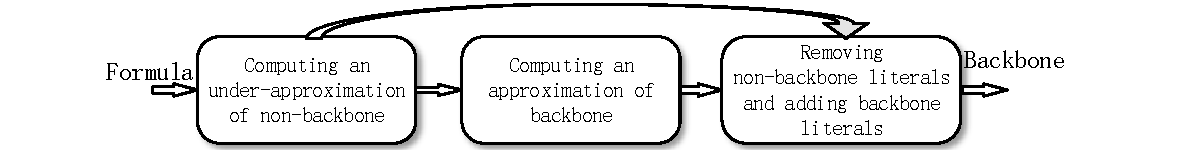
\includegraphics[scale=0.75]{Framework}
  \hspace*{-15mm} 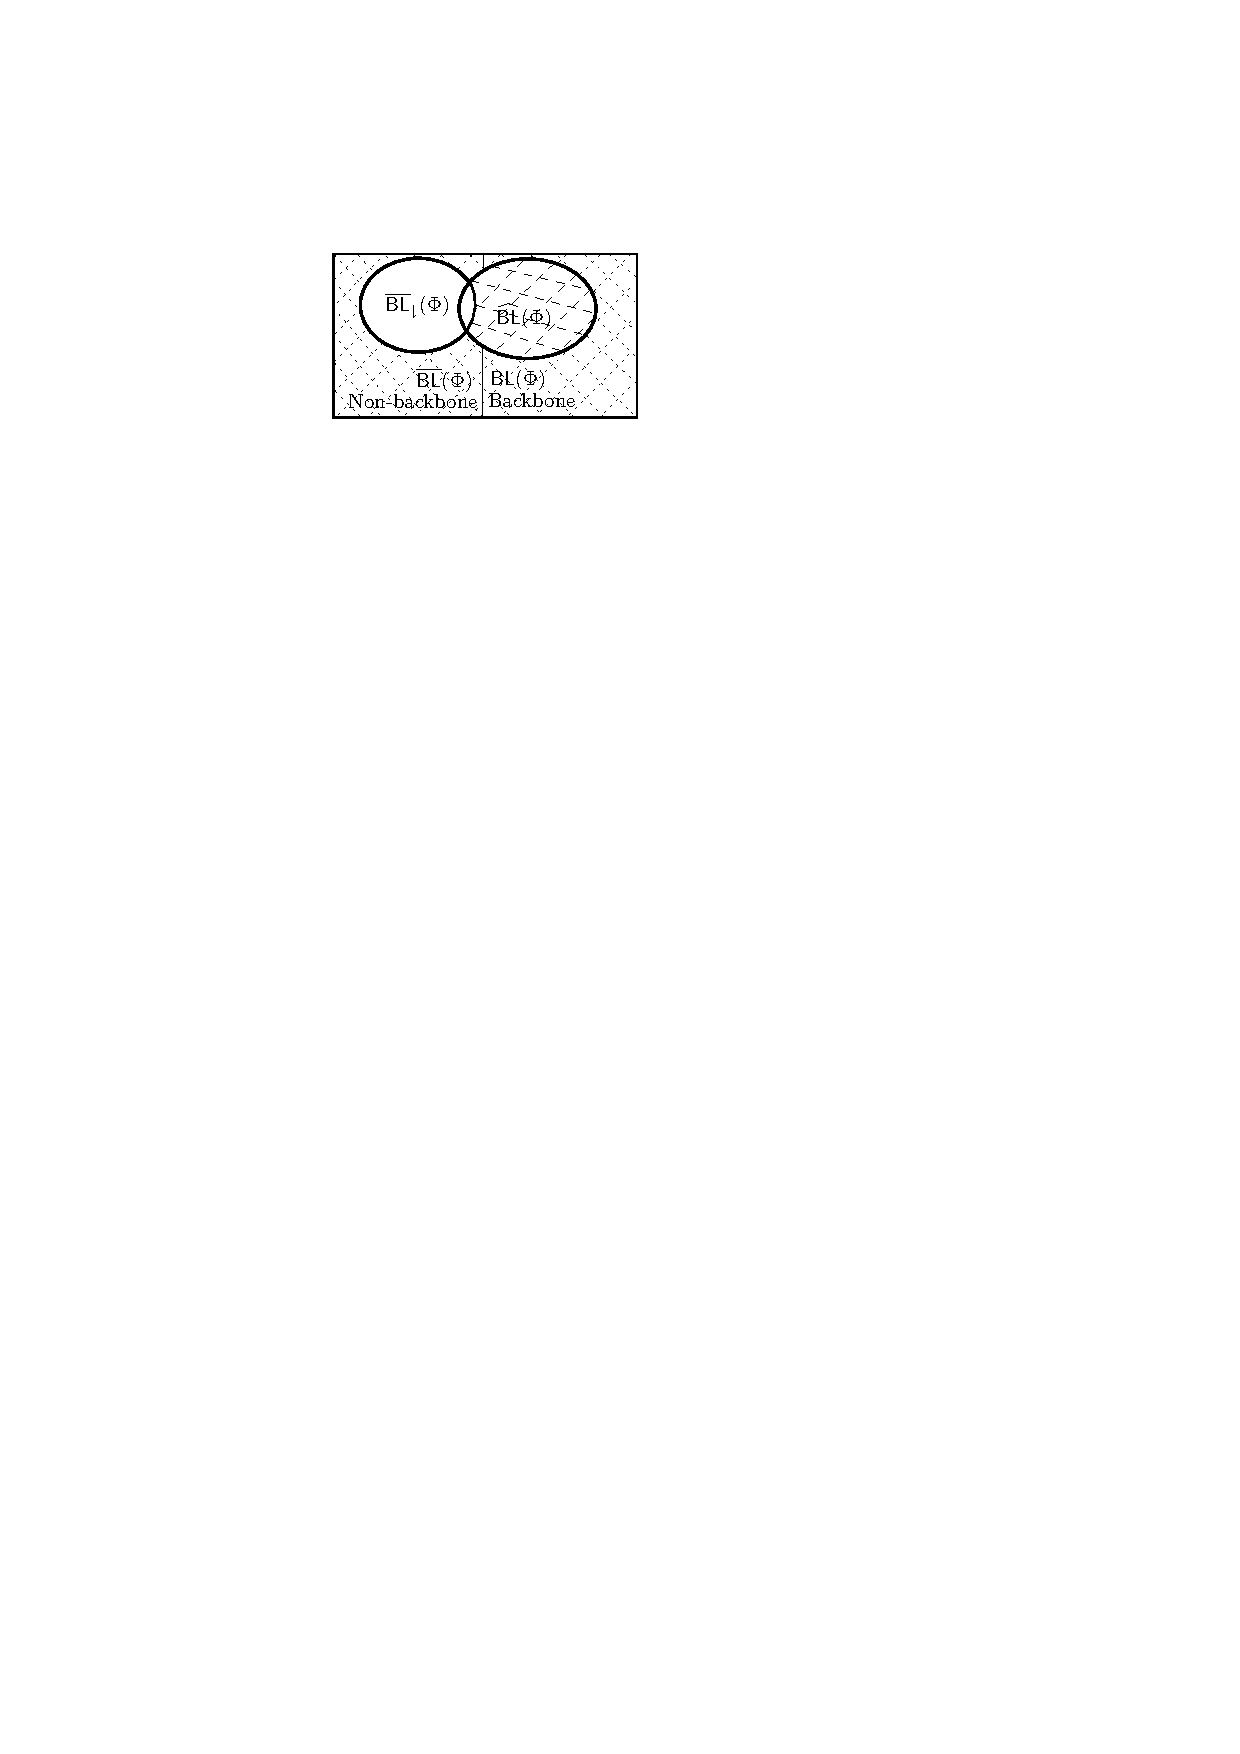
\includegraphics[scale=0.75]{Fig-backbone}
   \caption{Overview of our approach}
   \label{flow}
\end{figure*}

Figure \ref{flow} presents the overview of our approach \tool, which consists of three components. Taking a satisfiable formula
$\Phi$ as an input, \tool first computes an under-approximation $\NBLap(\Phi)\subseteq \NBL(\Phi)$ of the non-backbone of
$\Phi$. Then, \tool computes an approximation $\BLap(\Phi)$ of the backbone of $\Phi$ based on the set $\NBLap(\Phi)$, where each literal in $l\in \BLap(\Phi)$ has a high possibility to be a backbone literal of $\Phi$.
Finally, \tool removes non-backbone literals from $\BLap(\Phi)$ and adds backbone literals into $\BLap(\Phi)$ to compute the exact backbone of $\Phi$.

\medskip
\noindent{\bf Computing an under-approximation of non-backbone.}
Given a satisfiable formula $\Phi$, we first compute a model $\lambda$ of $\Phi$ by calling a SAT solver.
From the model $\lambda$, we compute a base under-approximation of non-backbone.
Later, we apply a Greedy-based algorithm to add more non-backbone literals into the base under-approximation, which results in the
under-approximation $\NBLap(\Phi)$.



\medskip
\noindent{\bf Computing an approximation of backbone.}
At this step, we apply an improved Whitening-based algorithm to compute the approximation $\BLap(\Phi)$.
The improved Whitening-based algorithm is an extension of the Whitening-based algorithm proposed by \cite{LMZ09} which
was used to compute \emph{frozen variables}, that are the variables whose values are fixed in a non-singleton set of models.
We use the Whitening-based algorithm of \cite{LMZ09} to compute the approximation $\BLap(\Phi)$. %which is then refined by
%a heuristic approach.


\medskip
\noindent{\bf Computing exact backbone.}
At this step, we use Algorithm 3 (Iterative algorithm) from \cite{JLM15} to compute backbone.
This algorithm uses SAT testing to check whether a literal is a backbone literal or not.
For instance, if $\Phi\vee \neg l$ is unsatisfiable but $\Phi$ is satisfiable, then $l$ must be a backbone literal of $\Phi$.


We first iteratively select one literal $l$ from $\BLap(\Phi)\setminus \NBLap(\Phi)$ such that $\lambda \models \neg l$ and test whether
$l$ is a backbone literal or not by checking the satisfiability of $\Phi\wedge l$ (dashed area in Figure \ref{flow}).
If $l$ is a backbone, we will add $l$ into $\Phi$ as a clause. Adding known backbone literals into $\Phi$ as clauses potentially speedups the later SAT testing \cite{JLM15,MPA2015}.
Then, we do the same testing for literals from $\Lit(\Phi)\setminus (\NBLap(\Phi)\cup\BLap(\Phi))$ (dotted area in Figure \ref{flow}).
After this step, the exact backbone and non-backbone are found.


In general, one can directly test all the literals to compute backbone without the two approximations.
However, the test heavily replies on SAT testing which may be time-cost.
Our approach makes two contributions compared to this na\"{\i}ve approach.
One is that we reduce the number of SAT calls using the known non-backbone literals $\BLap(\Phi)$.
The another one is that we first check literals that have high probability to be backbone literals so that backbone literals can be found as early as possible.



\section{Computing $\NBLap(\Phi)$}
In this section, we propose a Greedy-based algorithm that computes an under-approximation of non-backbone for a given formula
$\Phi$.

Given a formula $\Phi$ and a model $\lambda$ of $\Phi$, let $L(\Phi,\lambda)$
denote the set $\{l\in\Lit(\Phi) \mid \lambda\models \neg l \ \mbox{or} \  \forall \phi\in\Phi, l\in\phi\Rightarrow \exists l'\in\phi\setminus\{l\}: \ \lambda\models l'\}$.


\begin{lemma} \label{lem:navie}
 $L(\Phi,\lambda)\subseteq\NBL(\Phi)$.
\end{lemma}
Intuitively, suppose $l$ is a literal in $\Lit(\Phi)$ and $\lambda$ is a model of $\Phi$.
If $\lambda$ does not satisfy $l$, i.e.,  $\lambda\models  \neg l$, then $l$ must be a non-backbone literal of $\Phi$.
Otherwise, if $\lambda$ satisfies $l$ and for all clauses $\phi\in\Phi$, $\phi$ either does not contain the literal
$l$ or contains another literal $l'$ which is also satisfied by the model $\lambda$, then it is easy to see that
the assignment $\lambda[\neg l]$ satisfies $\Phi$.
In this case, $l$ is also a non-backbone literal.

However, $L(\Phi,\lambda)$ may excludes many other non-backbone literals.
To get more non-backbone literals, we propose the Greedy-based algorithm shown in Algorithm \ref{alg:greedy}.

\begin{algorithm}
\SetKwInOut{Input}{Input}
\SetKwInOut{Output}{Output}
\SetAlgoShortEnd
\SetFillComment
\Input{a satisfiable formula $\Phi$ and a model $\lambda$ of $\Phi$}
\Output{a set of literals $\NBLap(\Phi)$}
$\NBLap(\Phi):=L(\Phi,\lambda)$\; \label{alg1:init}
%\Repeat{No Update}{\label{alg1:loopstart}
\For{${\sf HS}$ from ${\sf HS}_1$ to ${\sf HS}_2$}{
    $C:={\sf HS}(\Phi)$\;
    $i:=0$\;
    \While{$i<|C|$}{
        $i:=i+1$,  $l:=C[i]$\;
        \If{$\lambda[\neg l]\models \Phi$}
        {
           $\NBLap(\Phi):=\NBLap(\Phi)\cup L(\Phi,\lambda[\neg l])$\;
           $\lambda:=\lambda[\neg l]$\;
        }
}
%    }

   % change the selected literal one by one to generate a new model\;
   % add new free literals to $\NBLap$.
    % $\Psi=\Psi\setminus\{\phi\in\Psi,\lambda(x)\models\phi, |\{l\in\phi \mid \l\models\phi\}|=2\}$\;
    % $\Psi=\Psi\cup\{\forall\phi\in\Phi, \neg\lambda(x)\models\phi\}$\;
    % $\lambda=\lambda[x\mapsto\neg\lambda(x)]$\;
    % $\NBL_i(\Phi)=\NBL_i(\Phi)\cup\{x\in\Lit(\Phi) \mid \forall\phi\in\Phi: \lambda(x)\models\phi\Longrightarrow\phi\in\Psi\}$\;
}\label{alg1:loopend}
\Return $\NBLap(\Phi)$\;
\caption{Greedy-based algorithm}
\label{alg:greedy}
\end{algorithm}
Given a satisfiable formula $\Phi$ and a model $\lambda$ of $\Phi$,
we assign $L(\Phi,\lambda)$ to $\NBLap(\Phi)$ at Line \ref{alg1:init}. Next, we update
$\NBLap(\Phi)$ using two heuristic searching strategies. % to select literalsat Lines \ref{alg1:loopstart}-\ref{alg1:loopend}.
Each heuristic searching strategy will give us a ordered set $C$ of literals, then select one literal by one literal from
$C$. For the select literal $l$, we obtain a new assignment $\lambda[\neg l]$ from the model
$\lambda$ and check whether  $\lambda[\neg l]$ satisfies $\Phi$ or not.
If $\lambda[\neg l]$ satisfies $\Phi$, then we add the set of non-backbone literals $L(\Phi,\lambda[\neg l])$ into $\NBLap(\Phi)$, and
assign $\lambda[\neg l]$ to $\lambda$ which will be severed as the model of $\Phi$ at the next step).
Obviously,  $\NBLap(\Phi)$ is an under-approximation of non-backbone of $\Phi$.

\begin{theorem}
$\NBLap(\Phi)\subseteq\NBL(\Phi)$.
\end{theorem}

Once, a model $\lambda$ of $\Phi$ is given, Algorithm \ref{alg:greedy} does not need to call any SAT solver which may be time-cost.
Instead, we manage to generate new models by changing assignments of literals in the known model.
We use the following two heuristic searching strategies to select literals. % with an order for generating new models.
\begin{quote}
Let $S$ be the ordered set of literals such that for every $i: 0\leq i<j<|S|$,
$f(\Phi,S[i])\leq f(\Phi,S[j])$, where $f$ is $\Cnt$ if $i=1$, and $f=\dens$ if $i=2$.
We define ${\sf HS}_i(\Phi)$ as the prefix sequence $S[0,xn]$ of $S$, for some $x\in[0,1]$.
\end{quote}

Intuitively, we choose the maximum $xn$ literals from the ordered set of literals.
The idea is that if the number $\Cnt(\Phi,l)$ of occurrence of a literal $c$ is smaller,
then the number of clauses that include the literal $l$ is smaller. This implies that the assignment $\lambda[\neg l]$ has a high probability to be a model of
$\Phi$. From the new model $\lambda[\neg l]$, we may find new non-backbone literals.
The intuition underlying ${\sf HS}_2(\Phi)$ is similar, in which we use densities of literals to sort literals instead of the numbers of occurrence.
The reason is that in longer clauses, there is a high possibility that the clauses can be satisfied by another literal. The longer the clauses are, the smaller the density of literal is. Therefore, literals with smaller density are more likely to give a new model of $\Phi$.




%\subsection{Heuristic-based Algorithm}

%With different models returned by MINISAT, the result of the algorithm in previous section diverged. To shrink the gaps, greedy based literals selection strategies are proposed. With a given literals selection strategy, a chain of literals can be complemented at the same time. In other words, a chain of models will be obtained by the changing assignments of literals, coverage of clauses for each literals are updated simultaneously. More models will be generated in this way.

%We apply a Greedy-Based Algorithm with different heuristic searching to extend the result of free literals and refereed as $\NBLap$. We leverages Greedy to depth first %searches. The quota we choose are frequency represented by the number of appearance of a literal and the entropy represented by the ratio of appearance number of a literal to %the total length of clauses that contains the literal. Each quota guided a Greedy search with maximal or minimal value.


%The algorithm take the free literals of a given model as input and assigned to $\NBLap$ as shown in Line 1. From Line 2 to Line 6, $\NBLap$ is expanded. Different heuristic %are chosen at Line 3 to select a list of literals and changing the assignment of them with a increased or decreased order.

%In order to generate different models from a given model, we need to negate more literals. We generate consecutive models by changing the assignments of literals one by one. %Since enumerating every model of a satisfied formula is known as a NP hard problem, many heuristic strategies are applied to model generation. The selection of literals paly %a vital role in it, with a different changing decisions, different models are generated. We take the idea of term frequency from statistic research, namely Term %Frequency-Inverse Document Frequency(TF-IDF). In our context, literals are regarded as terms, clauses are regarded as documents. The frequency of terms are represented as the %appearance number of literals. The inverse document frequency of a literal is represented as the ratio of appearance number to the total length of clauses that contained the %literal.

%\begin{lemma}
%The result of Algorithm \ref{alg:wal} is a subset of $\NBL$.
%\end{lemma}
%\begin{proof}
%For every model generated during the algorithms, the free literals is added to the result set of Algorithm \ref{alg:wal}.
%Since free literals is a subset of $\NBL$, the result is also a subset of $\NBL$.
%\end{proof}
% The final $\NBL_u(\Phi)$ result of our approach is $\NBL_u=\bigcup_{i=1}^4 \NBL_i(\Phi)\cup \NBL$.

% Compared with $\NBL_u(\Phi)$, the strategies applied in this sections can be viewed as four different kinds of depth-first search, while $\NBL_u(\Phi)$ is a width-first search. With different search methods, we are able to explore more paths and obtain more diverse models.

%<<<<<<< HEAD
%=======
%We propose two algorithms for computing $\NBL_u{\Phi}$. The first algorithm computing \MBNB.
%Second one \HBNB....
%We propose two algorithms for computing $\NBL_u{\Phi}$. The first algorithm computing \MBNB.
%Second one \HBNB....

%\MBNB computes a complete non-backbone literals set of a given model.
%It extracts the relation between literals and clauses, and generate a new model by applying single model rotation.
%The satisfiability of an assignment generated by single model rotation is related with the literal that complemented in the rotation. If a complementing a literal won't make any clause unsatisfiable, then a new model is generated. It's obvious that is there are at least two satisfied literal in a clause, then a new assignment generated by complementing one of the literals won't change the satisfiability of this clause. Therefore, by only complementing such literals, new models obtained from single model rotation.

%\HBNB computes extends the result of \MBNB with chain model rotation. With multiply rotations, we generate more models with from the initial model. It employs four heuristic depth first searches using Greedy strategies to find virous possible combinations of model rotation. The search is guided by the least/most coverage of literals which indicates the frequency of literals, and the maximal/minimal ratio of literals number to total length of clauses that contain the literal which indicated the importance of the literal to the formula.

%\medskip
%Based on $\NBL_u{\Phi}$, we apply optimized Whitening Algorithm to compute an approximation of backbone literals by eliminating one of the pattern that cause a false positive of Whitening Algorithm.
%We observe that Whitening Algorithm fail to recognize non-backbone literals when there is a large proportion of clauses that only have unique satisfied literal to a given model. We rule out non-backbone literals in this situation by distinguishing a special pattern among them. Among a group of clauses that only contain unique satisfied literal, there may exists a possible model rotation chain. By complementing the unique satisfied literal and more literals in each clause, another satisfied literal may emerge.
%....

%\medskip

% The basic idea is that if a clause is only satisfied by exactly one literal, no models can be obtained by only complementing the unique satisfied literal. Therefore, if a literal $l$ is not a unique satisfied literal for any clause, a new model $\lambda[l\mapsto\neg\lambda(x)]$ can be obtained. Literal $l$ is a non-backbone literal and will be added to $\NBL_u$.  Besides clauses-literals coverage analysis, we also propose different estimating strategies to extend and find more non-backbones. The strategies is a depth first search approach based on literals weights.
% We leverage whitening algorithm\cite{Par03,LMZ09} to extend the set of $\NBL_u$ to an estimation of backbones literals $\HDBS$ by complementing the result set of whitening algorithm. We refine $\HDBS$ iteratively by exploring model rotation chains. In the end, $\HDBS$ will be an estimation that literals in it are highly likely to be backbones.
%With $\NBL_u$, we are capable to estimate $\HDBS$. $\HDBS$ is initialized with the complement of $\NBL_u$, extensions are achieved by an iterative generation of a clauses estimation, called $\NBC$. For a clause $\phi$ that contains at least one literal $l\in\NBL_u$ or $\neg l \in\NBL_u$,  $\phi$ is added to $\NBC$. Given a model $\lambda$, for a literal $l\models\lambda, l\notin\NBL_u$, if $l$ appears in $\phi\notin\NBC$, $l$ is added to $\HDBS$.



%\subsection{An Na\"{\i}ve Algorithm}
%Definition.  Lemma.  Intuition. Proof.

%\begin{definition}[Free Literals of a Given Model]
%Given a formula $\Phi$, a model $\lambda\models\Phi$, a free literal $l\in\Lit(\Phi)$ is a literal such that a new model will generated by complementing $l$, i.e., %$\lambda[l\mapsto\neg l]\models\Phi$.
%\end{definition}

%\begin{lemma}[Free Literals]
%Given a formula $\Phi$, a model $\lambda\models\Phi$, a literal $l\in\Lit(\Phi)$ is a \emph{free literal} iff $\forall\phi\in\Phi, l\in\phi\wedge\lambda\models l %\Longrightarrow \exists l'\in\phi, l'\neq l\wedge\lambda\models l'$.
%\end{lemma}

%The satisfiable problem trying to find an assignment that satisfy each clause in a given formula. For a clause that satisfied by the given model, it will change to %unsatisfiable or maintain satisfiable when the model changes. We try to make every clause maintains satisfiable and generate a new model by negating the assignment of only %one literal.It's trivial that clauses will maintain satisfiable when the complementing literal doesn't appear in the clause. For clauses that contain the changing literal, %satisfiable will be maintained iff there is at least another literal which continues assigning the clause to TRUE. Therefore, if a literal only satisfy clauses that have at %least two satisfied literals, it's safe to conclude that it's a free literal.
%
%According to the definition of backbone, it's obvious that the set of free literals is a subset of $\NBL(\Phi)$.
%\begin{proof}
%\label{pro:free literal}
%Given a formula $\Phi$, a model $\lambda\models\Phi$.
%Suppose a literal $l\in\Lit(\Phi)$ is a free literal. If $l$ never shows up in any clause (trivial), then there is no such $\phi\in\Phi$ such that %$l\in\phi\wedge\lambda\models l$, $\exists l'\in\phi, l'\neq l\wedge\lambda\models l'$ always holds. If $l$ shows up in some clauses, then there is a new model %$\lambda[l\mapsto\neg l]\models\Phi$, no clause changes to unsatisfiable because of the changing of $l$. It means that $\forall\phi\in\Phi$, if $l\in\phi$, there must exists %another literal $l'\neg l$, assigning $\phi$ to TRUE. Therefore, $\forall\phi\in\Phi, l\in\phi\wedge\lambda\models l \Longrightarrow \exists l'\in\phi, l'\neq %l\wedge\lambda\models l'$.

%Suppose a literal $l\in\Lit(\Phi)$, if $\forall\phi\in\Phi, l\in\phi\wedge\lambda\models l \Longrightarrow \exists l'\in\phi, l'\neq l\wedge\lambda\models l'$, it means that %for every clause that containing $l$, the satisfiable will maintain when changing $l$ to its negation by $l'$. Therefore, there must exist a new model $\lambda[l\mapsto\neg %l]\models\Phi$.
%\end{proof}

%Whitening Algorithm can't be applied to backbones extraction directly because it suffers from the over-estimation of non-backbones, i.e, backbones can also be selected to the $\NBL_u(\Phi)$ by the Whitening Algorithm. To fix this defect, only a part of Whitening Algorithm is employed.
%Given a model $\lambda$, there is a possibility that more models can be obtained only by complementing several literals in $\lambda$ without calling a SAT solver. According to the theory of satisfiability, a model $\lambda$ is a truth assignment that satisfies every clause in the formula, i.e., there does not exist a clause $\phi$ that contains no literal in model $\lambda$. With a given model $\lambda$, non-backbones estimation approach is able to compute several similar models that only one literal in complemented. The literals that has been complemented are non-backbones.

%\begin{algorithm}
%\SetKwInOut{Input}{Input}
%\SetKwInOut{Output}{Output}
%\SetAlgoShortEnd
%\SetFillComment
%\Input{$\Phi$: a formula}
%\Output{$\NBLap(\Phi)$: under-approximation of non-backbones}

%$\Psi:=\NBLap(\Phi):=\emptyset$\;
%$(b,\lambda):=\SAT(\Phi$)\;
%\lIf{$b==0$} \Return $\Lit(\Phi)$\;
%$\Psi := \Psi\cup\{\phi\in\Phi \mid \exists l_1, l_2\in \phi, l_1\neq l_2 \wedge\lambda\models l_1\wedge l_2\}$\;
%$\NBLap(\Phi):=\{l\in\Lit(\Phi) \mid  \forall\phi\in\Phi: (\lambda\models l\wedge l\in\phi)\Longrightarrow\phi\in\Psi\}\cup \NBLap(\Phi)$\;
%\Return $\NBLap(\Phi)$\;
%\caption{Non-backbones under-approximation}
%\label{alg:no-loop-w}
%\end{algorithm}

%Given a formula $\Phi$, Algorithm \ref{alg:no-loop-w} computes a set of backbone literals $\NBL_u(\Phi)$ which is a under-approximation of $\NBL(\Phi)$.
%Algorithm \ref{alg:no-loop-w} maintains a set $\Psi$ of clauses and a set of candidate literals of $\NBL_u(\Phi)$, both of them are initialized to $\emptyset$ at Line $1$.
%At Line $2$, an off-the-shelf SAT Solver is called which returns a pair $(b,\lambda)$, where $b$ denotes whether $\Phi$ is satisfiable or not. If $b$ is TRUE, then $\lambda$ is an assignment that satisfies
%$\Phi$. If $b$ is FALSE, $\lambda=\emptyset$, Algorithm \ref{alg:no-loop-w} terminates and returns the set $\Lit(\Phi)$ at Line $3$.
%The Loop at Lines $4-6$ iteratively updates the sets $\NBL_u$ and $\Psi$ for each clause $\phi\in\Phi$. For each clause $\phi\in\Phi$, if there are at least two literals in %$\phi$
%that are satisfied by the assignment $\lambda$, then the clause $\phi$ is added into $\Psi$ at Line $5$. If there is a literal that only satisfy clauses in $\Psi$, the literal is added into $\NBL_u(\Phi)$ at Line $6$.

%\begin{lemma}
%Given a satisfied formula $\Phi$, a model $\lambda$. Let $\NBL(\Phi)$ be the non-backbones of $\Phi$.
%$x\in\Lit(\Phi), x\in\NBL(\Phi)$ iff $\exists\lambda'\models\Phi, \lambda\neq\lambda',
%\lambda(x)=\neg\lambda'(x)$.
%\end{lemma}\label{lem:nBL}
%\begin{proof}
%Suppose literal $x\in\Lit(\Phi)\in\NBL(\Phi)$, according to the definition of $\NBL(\Phi)$,
%it must exist two satisfied $\lambda, \lambda'\models\Phi$
%such that $\lambda(x)=\neg\lambda'(x)$, i.e.,
%$\forall x\in\NBL(\Phi)\Longrightarrow\exists \lambda\neq\lambda', \lambda(x)=\neg\lambda'(x), \lambda\models\Phi,\lambda'\models\Phi$.

%Suppose $\lambda, \lambda'$ are two satisfied assignments for a formula $\Phi$,
%$\lambda(x)=\neg\lambda'(x)$.
%According to the definition of $\NBL(\Phi)$, $x$ is in $\NBL(\Phi)$.
%\end{proof}

%\begin{theorem}
%Given a satisfiable formula $\Phi$, let $\NBL_u(\Phi)$ be the set of variables obtained by applying Algorithm \ref{alg:no-loop-w}, then $\NBL_u(\Phi)\subseteq\NBL(\Phi)$.
%\end{theorem}
%\begin{proof}

%Given a satisfied formula $\Phi$, a satisfied assignment $\lambda\models\Phi$.
%Suppose literal $x\in \NBL_u(\Phi)$, let $\Phi_{x}$ be the set of clauses that uses $x$.

%Since $\Phi$ is a satisfied formula, according to the theory of satisfiability, it must exist at least one model $\lambda\models\Phi$. It exists a model $\lambda'=\lambda[x\mapsto\neg\lambda(x)]$, $\lambda'\models\Phi\setminus\Phi_{x}$.
%For every clause $\phi\in\Phi_{x}$, there exists another ${x_1}$, $x\neq x_1$ such that $\lambda(x_1)\models\phi$ (Line $5,6$), $\lambda'(x_1)=\lambda(x_1)$ therefore $\lambda'\models\Phi_{x}$.
%For every clause $\phi\in\Phi_{\neg x}$, $\lambda(x)\not\models\phi$, it exists another ${x_2}$, such that $\lambda(x_2)\models\phi$ (Line $7$), $\lambda'(x_2)=\lambda(x_2)$, therefore $\lambda'\models\Phi_{\neg x}$.
%According to the above proof $\lambda'\models\Phi\setminus\Phi_{x}\cup\Phi_{x}\cup\Phi_{\neg x}=\Phi$.
%According to Lemma \ref{lem:nBL}, $\exists \lambda, \lambda'\models\Phi, \lambda(x)=\neg \lambda'(x)\Longrightarrow x\in\NBL(\Phi)$.
%\end{proof}

%In this section, we proved that there is no backbones in $\NBL_u(\Phi)$, it's safe to directly remove the literals in $\NBL_u(\Phi)$ from backbones estimation.


\section{Computing $\BLap(\Phi)$}
In this section, we propose an Whitening-based Algorithm to compute an approximation $\BLap(\Phi)$ of backbone.

\cite{Par03} proposed an Whitening algorithm which was supposed to determine nodes that always have the same color in all legal colorings of the coloring problem.
This algorithm was also used to compute (non-)frozen literals of model clusters in SAT problem \cite{LMZ09}, from which we can compute (non-)backbone literals.


\begin{algorithm}
\SetKwInOut{Input}{Input}
\SetKwInOut{Output}{Output}
\SetAlgoShortEnd
\SetFillComment
\Input{a formula $\Phi$ and a model $\lambda$ of $\Phi$}
\Output{white clauses $W_c$ and white variables $W_v$}
$W_c:= \{\phi\in\Phi \mid \exists l_1,l_2\in\phi: \  \lambda\models l_1\wedge l_2\}$\;
$W_v:=\{x\in \var(\Phi)\mid \lambda\models x\Rightarrow x\not\in \Lit(\Psi\setminus W_c),
        \ \lambda\models \neg x\Rightarrow \neg x\not\in \Lit(\Psi\setminus W_c)\}$\;
\Repeat{No Update of $W_c$ and $W_v$}{
   $W_c := W_c \cup \{\phi\in\Phi \mid \var(\phi)\cap W_v\neq \emptyset \}$\;
   $W_v := W_v \cup \{x\in \var(\Phi)\mid \lambda\models x\Rightarrow x\not\in \Lit(\Psi\setminus W_c),
        \ \lambda\models \neg x\Rightarrow \neg x\not\in \Lit(\Psi\setminus W_c)\}$
}
\Return $(W_c, W_v)$\;
\caption{Whitening algorithm}
\label{alg:whitening}
\end{algorithm}

Given a satisfiable formula $\Phi$ and a model $\lambda$ of $\Phi$,
Algorithm \ref{alg:whitening} computes a set of white clauses $W_c$ and white variables $W_v$ by iteratively making variables and clauses as white.
The remaining non-while variables give use an under-approximation of frozen literals in the model $\lambda$ of $\Phi$, namely,
$F(\Phi,\lambda)=\Lit(\Phi)\cap \{x,\neg x\mid x\in \var(\Phi)\setminus W_v(\Phi,\lambda)\}$ is a subset of frozen literals in the model $\lambda$ of $\Phi$.


Initially, all the clauses which contain at least two satisfied literals by $\lambda$ are marked as white.
Then, each variable $x$ whose value in $\lambda$ do not satisfy any non-white clauses is marked as white.
Intuitively, if $\lambda(x)$ is $1$ and the literal $x$ does not appear in any non-white clauses $\Phi\setminus W_c$, then $x$ is marked as white. In this case,
the assignment $\lambda[\neg x]$ satisfies all the non-white clauses, because no literal
$x$ appears in them, while the assignment $\lambda[\neg x]$ also satisfies white clauses, because there are at least two literals in each of white clauses
satisfied by $\lambda$. We get that the assignment $\lambda[\neg x]$ is a model of $\Phi$ which implies that $\lambda[\neg x]\in \cl_\Phi(\lambda)$.
On the other hand, if $\lambda(x)$ is $0$ and the literal $\neg x$ does not appear in any non-white clauses $\Phi\setminus W_c$, then $x$ is marked as white.
Since the assignment $\lambda[\neg x]$ satisfies all the non-white clauses thanks to the absence of the literal
$\neg x$ in them, and satisfies all the white clauses due to fact that there are at least two literals in each of white clauses satisfied by $\lambda$.
We still get that the assignment $\lambda[\neg x]$ is a model of $\Phi$ and $\lambda[\neg x]\in \cl_\Phi(\lambda)$.
Therefore, we can infer that if the variable is $x$ white, then the literals $\neg x$ and $x$ cannot be frozen literals.

Next, Algorithm \ref{alg:whitening} iteratively and alternatively marks each clause that contain at least one white variable and each variable whose value in $\lambda$ do not satisfy any non-white clause are marked as white, until no more clause or variable can be marked as white.
This loop manages to mark as many as variables as white [possible?].
After Algorithm \ref{alg:whitening} has terminated, if a variable $x$ is non-white, i.e., $x\not\in W_v$, then there does not exist a model $\lambda'\in \cl_\Phi(\lambda)$ such that $\lambda(x)\neq \lambda(x')$. This implies that the literal $x$ (resp. $\neg x$) is a frozen literal
in the model $\lambda$ if $x\in \Lit(\Phi)$ (resp. $\neg x\in \Lit(\Phi)$).  However, it was pointed out by \cite{LMZ09} that there are cases in which
a literal $l$ is not a frozen literal, but the corresponding variable $\var(l)$ is marked as white. We refer to \cite{LMZ09} for details.



\begin{theorem}\cite{LMZ09}
\label{thm:whiten}
$F(\Phi,\lambda)\subseteq\FL(\Phi,\lambda)$.
\end{theorem}


Given a satisfiable formula $\Phi$ and a model $\lambda$ of $\Phi$, we use $W_v(\Phi,\lambda)$ (resp. $W_c(\Phi,\lambda)$) to denote the set
$W_v$ (resp. $W_c$) obtained by Algorithm \ref{alg:whitening} taking $\Phi$ and $\lambda$ as inputs.


From Proposition \ref{prop:Frozen-backbone} (i.e., $\BL(\Phi)\subseteq\FL(\Phi,\lambda)$) and Theorem \ref{thm:whiten},
we can get that literals in $F(\Phi,\lambda)$ have high probabilities to be backbone literals. However, the set $F(\Phi,\lambda)$ also contains non-backbone literals. We propose a heuristic strategy that intends to remove non-backbone literals from $F(\Phi,\lambda)$.


Our strategy is based on the observation of the relationship between $W_c(\Phi,\lambda)$ and backbone literals.
Consider the formula $\Phi=(a\vee\neg b)\wedge(b\vee\neg c)\wedge(c\vee\neg a)$ and the model $\lambda$ such that $\lambda(a)=\lambda(b)=\lambda(c)=1$. The backbone of the formula $\Phi$ is $\emptyset$, because the assignment $\lambda'$ such that $\lambda'(a)=\lambda'(b)=\lambda'(c)=0$ is also a model of $\Phi$.
However, by Algorithm \ref{alg:whitening},
$W_v(\Phi,\lambda)=\emptyset$, from which we get that $F(\Phi,\lambda)=\Lit(\Phi)$. To remove the non-backbone literals $a, \ b, \ c, \ \neg a, \ \neg b$ and  $\neg c$
from $F(\Phi,\lambda)$,  we introduce a dependency graph to characterize such literals $a, \ b, \ c, \ \neg a, \ \neg b$ and  $\neg c$ from  the given formula $\Phi$.


Given a formula $\Phi$, the \emph{dependency graph} $G_\Phi$ of $\Phi$ is a undirected graph $(V,E)$, where
$V=\Lit(\Phi)$ is a finite set of vertices, and $E\subseteq V\times V$ is a finite set of edges which is defined as follows:
for every literals $l_1,l_2\in\Lit(\Phi)$, $(l_1,l_2)\in E$ iff one of the following conditions hold:
\begin{itemize}
\item there exists a clause $\phi\in\Phi$ with $l_1,l_2\in \phi$, 
\item  $l_1=\neg l_2$,  
\item $l_1=l_2\in\Phi$ (i.e., $l_1$ is a clause in $\Phi$).
\end{itemize}

It is easy to see that if a node $l$ has a self-cycle (i.e., $l\in\Phi$), then $l$ must be a backbone literal of $\Phi$.
Figure \ref{fig:depend} depicts the dependency graph of the formula $(a\vee\neg b)\wedge(b\vee\neg c)\wedge(c\vee\neg a)$.
 \begin{figure}
    \centering
    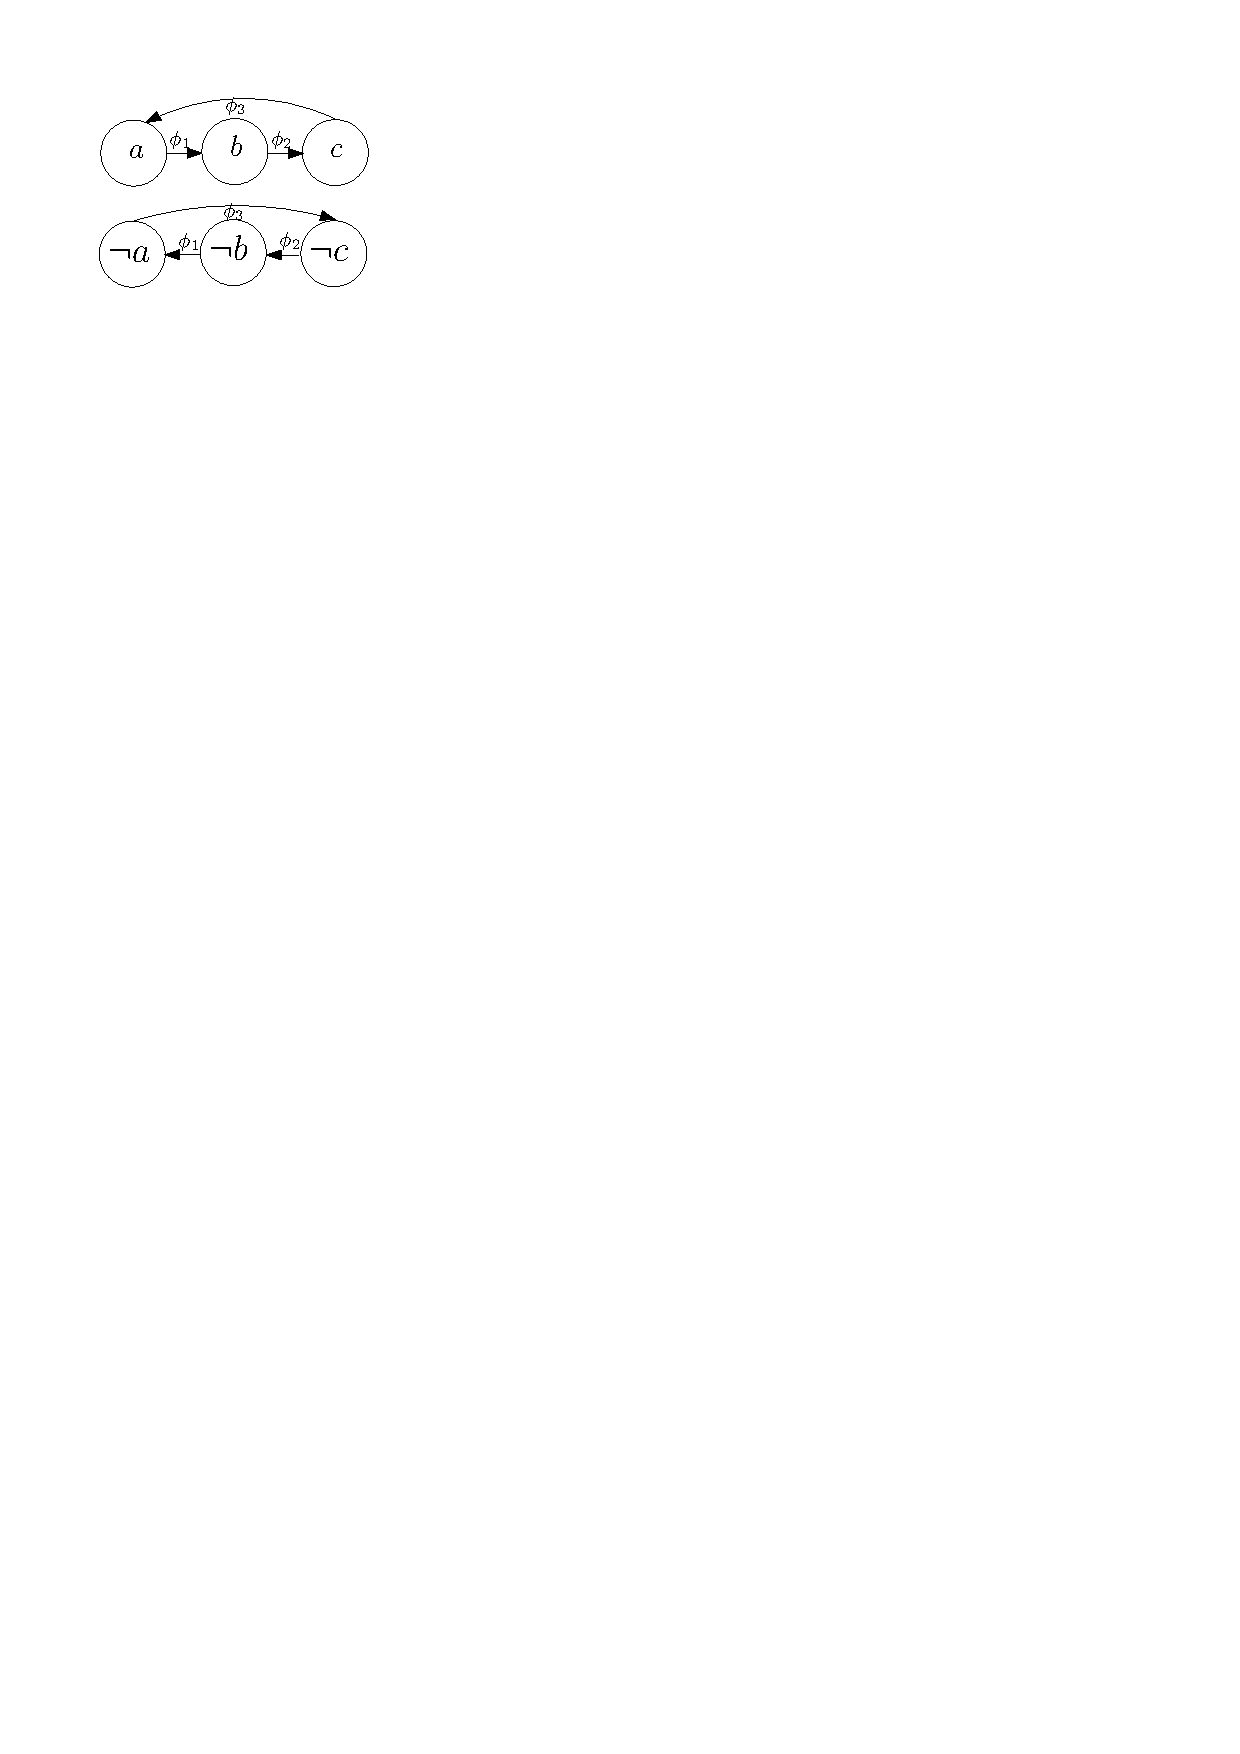
\includegraphics[scale=0.7]{dependency.pdf}
   \caption{Dependency graph of $(a\vee\neg b)\wedge(b\vee\neg c)\wedge(c\vee\neg a)$}
   \label{fig:depend}
\end{figure}

A \emph{path} $\pi$ of a dependency graph  $G_\Phi=(V,E)$ is a sequence $l_1...l_n$ of nodes, such that for every $i:\ 1\leq i<n$, $(l_i,l_{i+1})\in E$.
We use $\Lit(\pi)$ to denote the set of literals appeared in $\pi$ and $E(\pi)$ to denote the set of edges used in $\pi$.
Let $\Phi_\pi$ denote the set of clauses $\{\phi\in\Phi\mid \exists (l,l')\in E(\pi): l,l'\in \phi\}$.

A path $l_1l_2...l_n$ is \emph{valid} if $n>2$ and $|\var(\bigwedge_{1\leq i\leq n} l_i)|\geq 2$, i.e., there are at least two different variables used in
the literals  $l_1,l_2,...,l_n$. Let $\Pi(l)$ denote the set of all the valid paths starting from $l$.
A path $l_1l_2$ is \emph{trivial} if $l_1=\neg l_2$ or there exists a clause $\phi$ such that $l_1,l_2\in\phi$.
%A path $\pi=l_1...l_n$ is a \emph{pure clause path} if $l_1,...,l_n\in \Lit(\Phi_\pi)$ and $l_1,...,l_n\not\in \Lit(\Phi\setminus\Phi_\pi)$.
A valid path $l_1...l_{2n}$ is \emph{mutable} if $l_1=\neg l_{2n}$, for every $1\leq k < n$, $l_{2k}=\neg l_{2k+1}$.

\begin{proposition}
Given a model $\lambda$ of $\Phi$ and a valid mutable path $\pi$ in $G_\Phi$, 
suppose $L(\pi)=\{l_1,...,l_n\}$,  then the assignment $\lambda[\neg l_1]...[\neg l_n]$ satisfies $\Phi_\pi$.
\end{proposition}
 
Given a literal $l\in \Lit(\Phi)$, if there does not exist any valid mutable path $\pi\in\Pi(l)$, then $l$ must be a non-backbone literal.


Given a literal $l\in \Lit(\Phi)$, if for every $l'$ such that $l,l'\in \phi$ for some $\phi\in\Phi$,
there exists valid mutable path $\pi\in\Pi(l')$, then $l$ must be a non-backbone literal.
  
 
 For every path in $\Pi(l)$, if $\Lit(\Pi(l))\setminus\{l\}$ is non-backbone literals and a new model formed when complementing every literal on the path simultaneously, then $l$ is a non-backbone literal.

 Such non-backbone checks of literals may be nested due to the dependency of literals. Therefore, instead of checking every literal in a path, we use the counterexample idea, if there exists a path $\pi$ in $\Pi(l)$, that $\Phi_{\pi}$ will be unsatisfied when complementing every literal in $\Lit(\pi)$ at the same time, then there is no immediate model from mutating a path starting from $l$.

 However, with the help of SAT solver, it's still possible to generate a model by complementing a literal that doesn't have a immediate model from mutating a path. A Mutate path just implies one possible set of literals which complementing simultaneously to generate a new model, other sets of literals are still available to generate new models.

 [Explanation]For valid paths, we want to check the possibility that complementing the literals on paths simultaneously. Given a path $\pi$, we use $\pi[i]$ to denote the $i_{th}$ literal on the path. Suppose a path with a length of four literals, $x, \neg y, y, \neg x$ respectively. It implies that $x$ and $\neg y$ are in the same clause $\phi_1$ and $y, \neg x$ are in the same clause $\phi_2$. It's obvious that both $\phi_1$ and $\phi_2$ are still satisfy by the new assignment $\lambda[\neg x, \neg y]$ from the path. The assignment $\lambda[\neg x, \neg y]$ will be a new model if $\Phi_x$ and $\Phi_y$ are either white clauses or clauses labeled in a such path. More generally, if a path with length k, contains several complementing pair of literals started from $\pi[2]$ to $\pi[k-1]$, it is refereed as \emph{mutate path}. A new assignment $\lambda[\neg l, l\in\{\pi[i] | l\in[2, k-1]\}]$ will satisfy the labeled clauses in this path. If $\Phi_l$, $l\in\{\pi[i] | l\in[2, k-1]\}$ are all white clauses or clauses labeled in a mutate path, a new model is obtained from the path.Our approach applying the counterexample idea to the facts presented above, consider a literal $l\in F(\Phi, \lambda)$ if there is a non-mutate path starting from $l$, we consider that there is no immediate model generated the literal $l$.
 However, it's possible to obtain a new model by complementing the literal that have a non-mutate path. But it's usually time-cost. In order to avoid calling SAT solvers, our approach just remove the literals that have an non-mutate path. We will apply an iteratively SAT testing Algorithm to deal with this literals.


\begin{algorithm}
\SetKwInOut{Input}{Input}
\SetKwInOut{Output}{Output}
\SetAlgoShortEnd
\SetFillComment
\Input{$\Phi$: a formula, $\NBLap$: under-approximation of non-backbone}
\Output{$\BLap(\Phi)$: backbone approximation of $\Phi$}

$\BLap:=F(\Phi, \lambda)\setminus\{l | \forall \pi, \pi[1]==l\Longrightarrow\pi[2k]==\neg\pi[2k+1], k\in[2,n-1]\}$\;
%\For{$l\in\BLap(\Phi)$}{
%    \For{$\phi\in\Phi_l$}{
%        $found:=TRUE$\;
%        $k:=1$\;
%        $\Phi_{l}^0:=\{l\}$\;
%        \Repeat {$\Phi_{l_l}^k==\Phi$}{
%            $\Phi_{l}^k:=\{\phi\in\Phi \mid \neg\Lit(\Phi_{l}^{k-1})\in\phi\}$\;
%            \If{$\neg l\in\Lit(\Phi_{l}^k)$}{
%                    break\;
%            }
%            $k++$\;
%        }
%        \If{$\Phi_{l_l}^k==\Phi$}{
%            $found:=FALSE$\;
%            break\;
%        }
%    }
%    \If{found}{
%        $\BLap(\Phi):=\BLap(\Phi)\setminus\{l\}$\;
%    }
%}
\Return $\BLap(\Phi)$\;
\caption{Backbones approximation of $\Phi$}
\label{alg:nBLo}
\end{algorithm}

Algorithm \ref{alg:nBLo} works on the dependency graph of a formula. For each literal in $F(\Phi, \lambda)$ it find all valid paths starting from the literal. If every valid path is a mutate path for the literal, then it's removed from $\BLap$. Otherwise, the literal is kept in $\BLap$ since there may not exist a model generated from complementing the literal.

Given a satisfiable formula $\Phi$, the dependency graph of $\Phi$ is $G(\Phi)$. Algorithm \ref{alg:nBLo} computes a approximation of backbone literals $\BLap$ by checking paths in $G$ started from a literal $l\in F(\Phi, \lambda)$ is a mutate path or not. If there is a not mutate path starting from literal $l$, $l$ is removed from $F(\Phi, \lambda)$.

After Algorithm \ref{alg:nBLo} has terminated, if a literal is in $F(\Phi, \lambda)$, we consider that there is a higher probability for the literal to be a backbone literal.


\section{Experimental Study}\label{sec:expr}
We implemented our approach in a tool called \tool written in C++ interfacing Minisat 2.2 \cite{MINISAT}.
In this section, we present the experimental results of \tool.
The benchmark consists of two parts: 388 industrial formulae and 6606 random formulae.
The experiments were conducted on a cluster of IBM iDataPlex 2.83 GHz, each instance was running with a timeout of 1800s and memory limit of 8GB.
The experimental results demonstrate that \tool outperforms the  state-of-the-art backbone computing tool
\textit{cb100} \cite{JLM15}. \tool and our benchmark are available at \url{https://github.com/bone-tool}.

\subsection{Benchmark Setup}
The benchmark consists of two parts: 388 industrial formulae and 6606 random formulae.
Industrial formulae were selected from SAT competitions between 2002 and 2015.
There are 1318 formulae in all these benchmarks containing random formulae or crafted large formulae.
Among them, there are 769 formulae from industrial verification including planning, coloring, hardware/software verification, model checking and cryptanalysis.
As only satisfiable formulae make sense for computing backbone, we chose 388 formulae from 769 formulae that are satisfiable using MiniSat under 1800s.


To evaluate the scale  of \tool, we design an interesting approach to generate about 6600 \textit{random} formulae using 100 unsatisfiable formulae as the seeds. We have the fact that for each unsatisfiable formula $\Phi$, we can find the \textit{maximal satisfiable subset} $\Psi\subset \Phi$
iff $\Psi$ is satisfiable and for every clause $\phi\in\Phi\setminus \Psi$, $\phi\wedge \Psi$ is unsatisfiable.
Each maximal satisfiable subset is regarded as a satisfiable formula.
For a given unsatisfiable formula $\Phi$, there may exist more than one maximal satisfiable subsets of $\Phi$. Based on this idea, we use the tool LBX \cite{MPA2015} to generate 6606 maximal satisfiable subsets from which 100 unsatisfiable formulae randomly selected.





%In Table \ref{tab:ind}, it shows the results of industrial formulae. In Figure \ref{fig:ind-time}, it shows a plot by increasing running time of industrial instances for \tool and \textit{cb100}. We make the random benchmark into 3 groups, according to the community structure of the formula. In Table 3, it shows the result of random formulae, including total SAT solving time, average SAT solving time and average SAT solver call for all 3 groups and the whole benchmark.


\subsection{Experimental Results on Industrial Formulae}

\begin{table}[t]
\centering
\begin{tabular}{ccccc}
\toprule
 &Total  Time (s) & SAT Calls&Average Time (s)\\
\midrule
\tool&26663  &272089&0.9890  \\
cb100&30295  &239112&1.0174  \\
\bottomrule
\end{tabular}
\caption{Experimental results for 138 industrial formulae}
\label{tab:ind}
\end{table}

Table \ref{tab:ind} shows the overview of experimental results on industrial formulae.
Among all the 388 industrial formulae, there are 138 formulae that both \tool and \textit{cb100} were able to compute backbone within 1800s.
Although, the number of SAT calls used by \tool is greater than \textit{cb100}, \tool reduces by 12\% of the total running time and by 11\% of the average running time for each SAT call.

Figure \ref{fig:ind-time} provides the details of experimental results on industrial formulae, including the running time of the SAT solver for generating the first model and total running time for each formula.
The red dotted line represents for the time used by the SAT solver for computing the first model, which indicates the hardness of the formula.
Lines with crosses represents for the running time of \tool, and lines with boxes represents for the running time of \textit{cb100}. There is a correlation between the hardness of formulae the performance of \tool comparing to \textit{cb100}.
For most of hard formulae, \tool outperforms \textit{cb100} in terms of total running time and average time of each SAT solver call. This demonstrates that \tool is more feasible for computing backbone of hard formulae.

%\textit{cb100} highly rely on the quality of model returned by SAT solver, it performances better when SAT solver gave it a suitable model. For most of the formulae that need less than 1 second to compute a first model, both \tool and \textit{cb100} were able to compute backbone very quickly with barely difference.

Table \ref{tab:ind} and Figure \ref{fig:ind-time} demonstrate that \tool outperforms \textit{cb100} on industrial formulae.


\begin{figure}
    \centering
    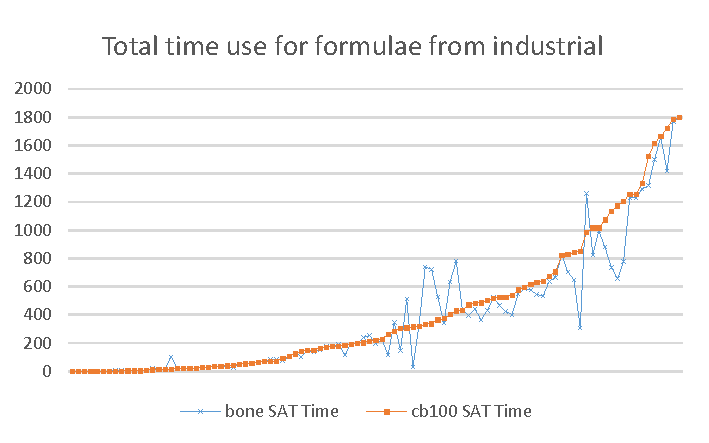
\includegraphics[scale=0.8]{ind2.pdf}
   \caption{Experimental results on industrial formulae}
   \label{fig:ind-time}
\end{figure}

\subsection{Experimental Results on Random Formulae}
In this section, we present experimental results on random formulae. Before presenting the overview of the experiments of the whole random formulae, we tested 100 random formulae from 6606 ones, which leads to finding what kind of formula are suitable to be solved by \tool.

\begin{figure}
    \centering
    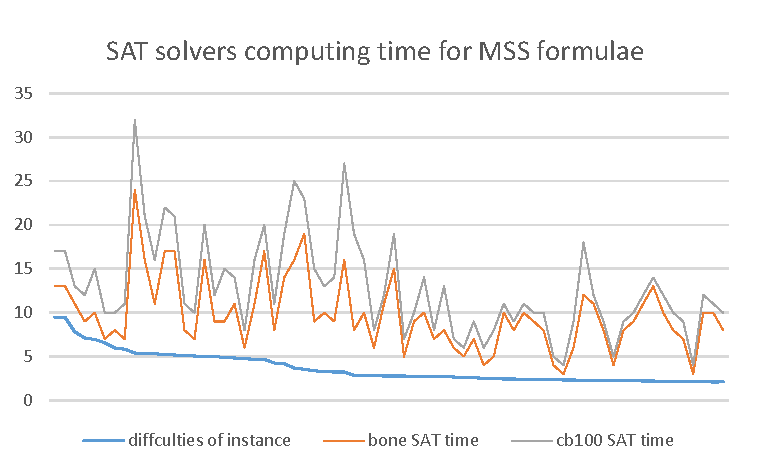
\includegraphics[scale=0.8]{mcs.pdf}
   \caption{Overview of results on industrial formulae}
   \label{fig:mcs-time}
\end{figure}

\begin{figure}[t]
\centering
\subfloat[cb100 performs better]{

\centering
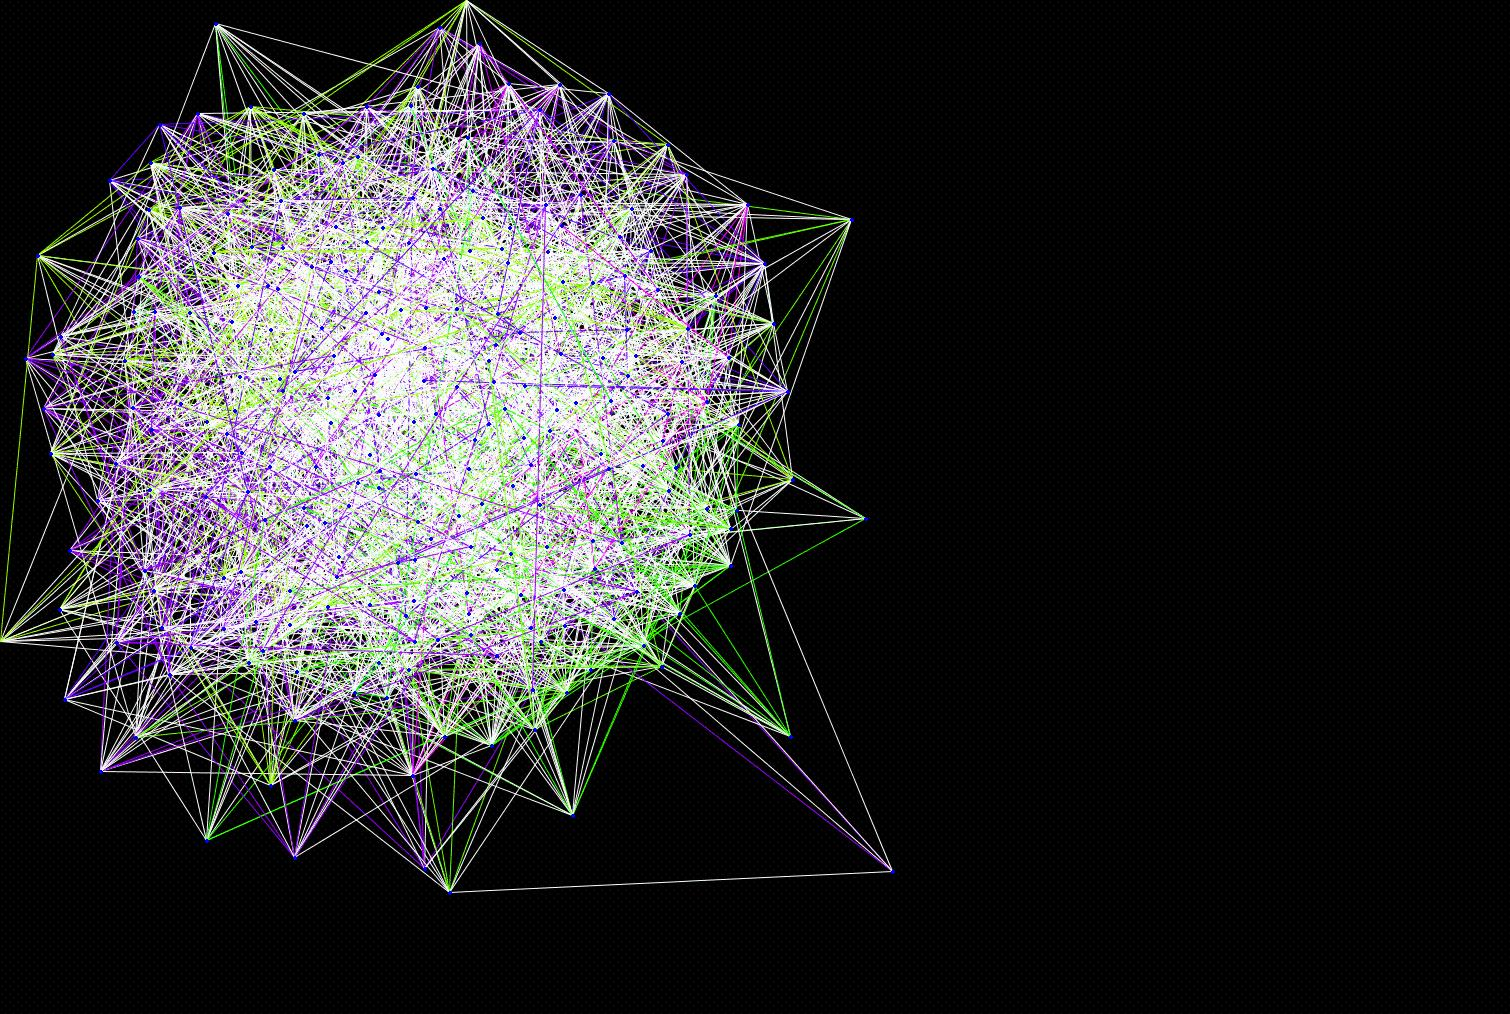
\includegraphics[width=.5\linewidth-0.45mm]{cb100.jpg}
}
\subfloat[\tool performs better]{
\centering
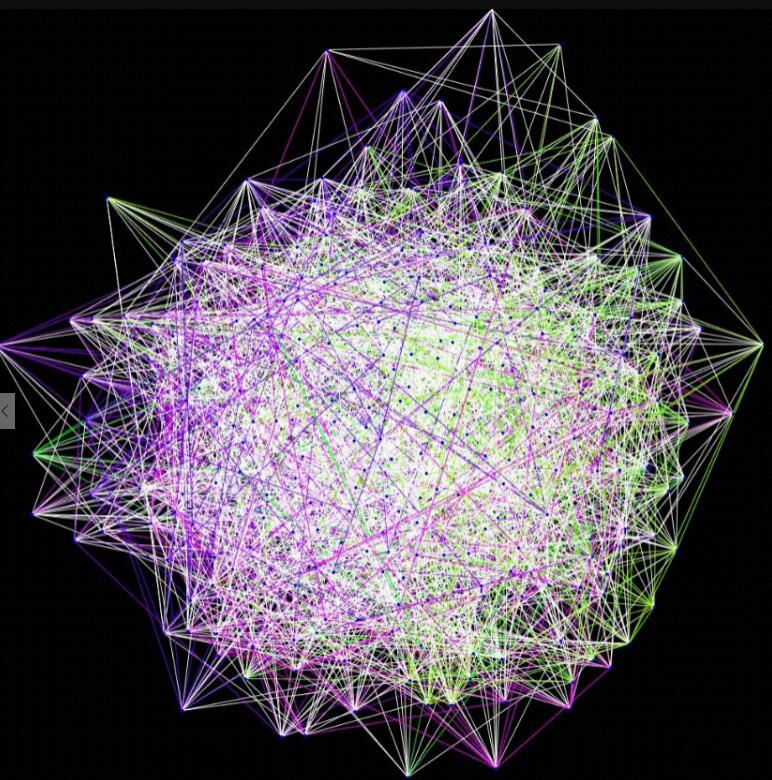
\includegraphics[width=.5\linewidth-0.45mm]{bone.jpg}
}
\caption{Community structures}
\label{fig:cs}
\end{figure}

\begin{table*}[!htb]
\begin{tabular}{c|c|c|c|c|c|c|c|c}
\hline
\multirow{2}{*}{} & \multicolumn{2}{c|}{Simple} & \multicolumn{2}{c|}{Medium} & \multicolumn{2}{c}{Hard}& \multicolumn{2}{|c}{Total} \\
\cline{2-9}
  & SAT Time (s) & SAT Calls & SAT Time (s)& SAT Calls & SAT Time (s)& SAT Calls&SAT Time (s)& SAT Calls \\
\hline
\tool& 6874.5   & 85570 & 35853   & 1332334 & 3577.9   & 76449  & 50183.02   & 1508723 \\ \hline
cb100 & 4413.5   & 86232 & 39040   & 1353258 & 5893.4   & 78114& 50414.04   & 1532372  \\
\hline
\end{tabular}
\caption{Results of random formulae}
\label{tab:mcs-graph}
\end{table*}
Figure \ref{fig:mcs-time} depicts the running time of results on  randomly formulae.
%selected 100 random formulae out of 6606 whose time of computing the first model range from 0s to more than 4s.
This result demonstrates that there is no correlation between the running time of backbone computing and running time of computing the first model, which is different from the result on industrial formulae. The reason is that random formulae have more complex community structures \cite{NZG2014,LJG2015SAT,LJG015}. Therefore, we cannot use running time of computing the first model to measure how hard a formula is.
To measure hardness of random formulae, we investigated community structures of all the random formulae, as it is already known that community structure of a formula affects the performance of conflict-driven clause learning based SAT solvers \cite{NZG2014}.


We constructed the community structures of all the random formulae using use SATGraph \cite{NZW2015}.
We observed that \textit{cb100} performs better on formulae whose community structures are divergent, i.e., there are vertexes far from the center of structures.
Figure \ref{fig:cs}(a) shows the community structure of one formula on which \textit{cb100} performs better.
While \tool performs better on formulae whose community structures are focusing.
Figure \ref{fig:cs}(b) shows the community structure of one formula on which \tool performs better.



Based on this observation, we divide 6606 random formulae into three groups according to their community structures.
The \emph{simple group} contains 371 formulae whose community structures are divergent,
the \emph{hard group} contains 337 formulae whose community structures are focusing,
and the \emph{medium} group contains 5898 formulae between divergent and focusing.


Table \ref{tab:mcs-graph} shows the experiments results on these three groups. \textit{cb100} performs better than \tool on the simple group, as \textit{cb100} tries to find a backbone literal by complementing models as soon as possible, which are the vertexes far from the center.
\tool outperforms \textit{cb100} for both medium group and hard group.
\tool reduces by 8\% for medium group and by 40\% for hard group of the total running time.


%\begin{figure}
%    \centering
%    \includegraphics[scale=0.2]{\textit{cb100}.jpg}
%   \caption{Community Structure of Formula Performs better with \textit{cb100}}
%   \label{fig:\textit{cb100}}
%\end{figure}

%\begin{figure}
%    \centering
%    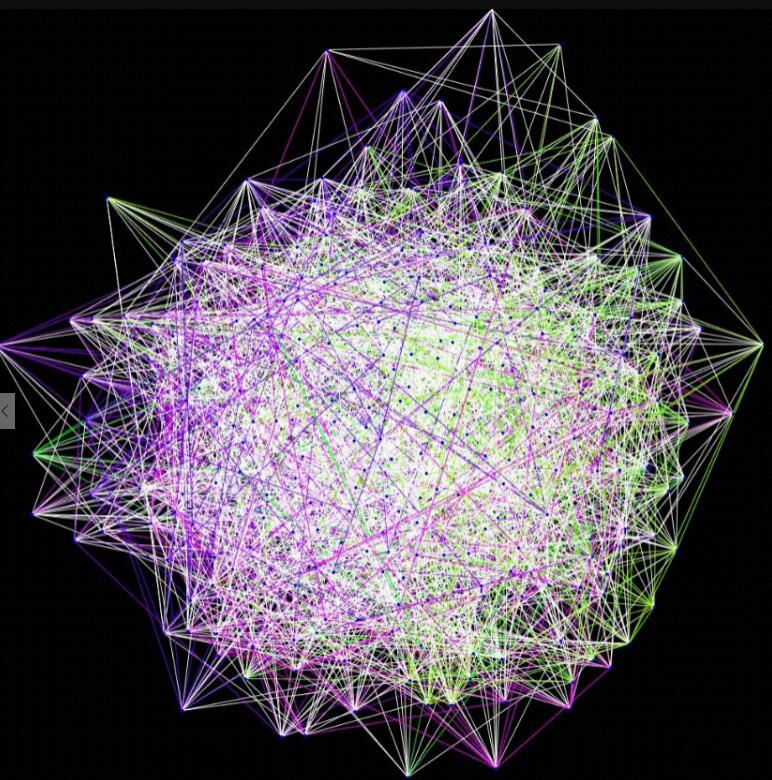
\includegraphics[scale=0.2]{bone.jpg}
%   \caption{Community Structure of Formula Performs better with \tool}
%   \label{fig:bone}
%\end{figure}


The experimental results show that \tool performs better than \textit{cb100} on hard random formulae and is comparable to \textit{cb100} on simple formulae.





\section{Related Work}\label{sec:relw}
% This paper is concerned with computing backbones of propositional formulae, which was oriented from coloring problem \cite{CJG2001}, with a wide range of practical applications such as MaxSAT \cite{MMBM2005}.

A number of backbones extraction algorithms have been proposed in recent years.

Monasson et al. reported an analytic solution and experimental investigation of the phase transition in K-SAT \cite{MZKST99}, in which
backbones play in an important role. This work showed that the presence of a `backbone' provides a good explanation for the apparent inevitably high cost of heuristic search near the phase boundary. Kaiser and K\"{u}hlin proposed three model enumeration based algorithms for computing backbones \cite{KKW2001}.
The first one iteratively assigns true (false) to each variable and tests the resulting formula for satisfiability.
The second one reuse the results of previous satisfiability checks and the last one maximizes the number of variables that
an be classified without satisfiability checking, which share same purpose as our work.

Dubois and Dequen proposed a heuristic search for computing Backbones of hard 3-SAT formulae which yields DPL-type algorithms with a significant
performance improvement over the best previous algorithms \cite{DD2001}.
Climer et al. proposed a graph-based approach to discover backbones which replies on approximate lower and upper bounds to compute
backbones of instances of the travelling salesman problem \cite{CZ2002}. 


Kilby et al. showed that backbones are hard even to approximate and proposed algorithms for computing backdoors, that are literals/variables whose absence will simplify formulas to be solved in polynomial time \cite{KPS2005}. As discussed by \cite{KPS2005}, backbones have little overlap with backdoors.

 

Zhu et al, proposed an iterative SAT testing based algorithm \cite{ZWSM11,ZWM11} which is more efficient than previous model enumeration. At the first step, this algorithm assigned the first model returned from SAT solver to backbone estimation, which need less memory to compute backbone.

Marques-Silva et al.  investigated algorithms for computing backbones emphasizing the integration of existing algorithms which include model enumeration, iterative SAT-testing and filtering with modern SAT solvers, as well as optimisations. 
They conducted an experimental evaluation of existing techniques and showed that backbone computation for large practical formulae is feasible. \cite{MJML2010,JLMS12,JLM15}. 
This work proposed a novel Greedy-Whitening based approach \tool.
Experimental results demonstrated that our approach performs better than the best one of algorithms in \cite{MJML2010,JLMS12,JLM15} for industrial formulae and
hard random formulae, while for simple formulae, \tool is also comparable.


 

 
%The algorithm maintained an estimation of backbone. In each iteration, a clause that formed by the negation of backbone estimation is added to $\Phi$. If $\Phi$ was satisfiable, it implied that at least one non-backbone literal is in the backbone estimation. Intersection between the model given by SAT solver and the backbone estimation indicates the non-backbone literal. In this way, non-backbone literal is removed, the process is repeated until $\Phi'$ is not satisfiable any longer. Along with the estimation, the clauses number of $\Phi$  is monotone increasing due to the continuously insertion in each iteration, which dramatically promote the complexity of $\Phi$. In other words, for each iteration, it takes longer CPU time than the last iteration.

%Janota et al, proposed an Iterative algorithm (one test per variable) \cite{JLM15}. For each iteration, it added only one unit clause to the original formula, which made the new formula easier. Inspired by this algorithm, our approach in this paper follows this idea.

%The Core Based Algorithm presented in \cite{JLM15} is stable and effectiveness. The cb100 tool, as our main comparative object, was based on this algorithm. %Instead of adding only one unit clause to the original formula, this algorithm added all the unit clause to the formula. It will dramatically accelerate SAT solving. Although there is a high possibility that the new formula is unsatisfiable, whenever there was only one literal in unsatisfiable reason of the new formula, this literal is a backbone literal. In this way, it was able to find backbone literals with little cost. In this paper, the author showed that for formulae with backbone percentages lower than 25\%, Core Based Algorithms are better.
%significantly better. When the percentage of backbone is over 25\%, Core Based Algorithm behave very similarly Iterative SAT Testing Algorithm.


%Kilby et al proposed \cite{KST2005} that there was little overlap between backbone and backdoors.

%In \cite{KKW2001}, they partitioned backbone into inadmissible and necessary group. For inadmissible group, literals were false in each satisfying variable assignment. For necessary group, literals were true in each satisfying variable assignment. They described and compared three algorithms for searching the set of necessary and inadmissible variables, a basic iterative testing and two enhancements. The first enhancement was reusing the result of satisfiability checks to get more models for free, the second enhancement was selecting the decision variables for SAT solvers according to the previous information of inadmissible and necessary group.


%In \cite{DOG2001}, they proposed a heuristic search for backbone, and choose this backbone variables as branch nodes for the tree developed by a DPL-type procedure. Experiments showed that a significant performance improvement over the best current algorithms, and enhanced the scalability of the algorithm up to 700 variables.

%In \cite{WS2001}, they concluded the correlation of backbone size with the problem of optimization and approximation, using graph coloring, Travel Salesman, Number partition and block words planning. And they suggested that it is necessary to eliminate trivial cases of backbone before using backbone size to evaluate the hardness of optimization and approximation problems.


\section{Conclusion}\label{sec:conc}
This paper develops improvements to algorithms for backbones extraction.
It's devises new preprocessing techniques for backbones extraction by computing under-approximation of backbones and non-backbones.
In addition, the paper implemented FCB and compared with CB with formulae from MCSes extraction, practical applications and 4 groups of formulae with a fixed percentage of backbones.

The experimental results indicate that FCB is able to reduce the SAT calls number as well as shorten the CPU time cost by a single SAT call.
However, for some of the formulae, CB needs less SAT calls than FCB does, which opening a possibility for portfolio-based solvers.
In other words, a suitable model will reduce the SAT calls number for both CB and FCB.

In the future, we plan to explore more practical applications for backbones, such as hardware model checking, SAT model counting and SAT model enumeration.

\newpage


\newpage
\bibliography{bib}
\bibliographystyle{aaai}

\end{document}
